
\chapter[\textbf{The Radius, Time, and Temperature Plot}]{: \ The RTT Plotting Function}
\label{app:rtt}
The Radius, Time, and Temperature (RTT) Plotting Function is a tool used to create common plots for 1-D Lagrangian Radiation-Hydrodynamics codes, like Bucky.  The Radius and Time refer to the ordinate and the abscissa of the 2-D plot, respectively, while the Temperature is in reference to a 2-D Variable's color plot that is overlaid on top of the underlying Radius Vs. Time plot (see Fig.\,\ref{fig:basePlot}).  The Radius Vs. Time Plot is the fundamental plot for 1-D Lagrangian Codes because it represents its two computational dimensions: space, by radius, and time.

\sidecaptionvpos{figure}{c}

\begin{SCfigure}[][h!]	
	\centering
	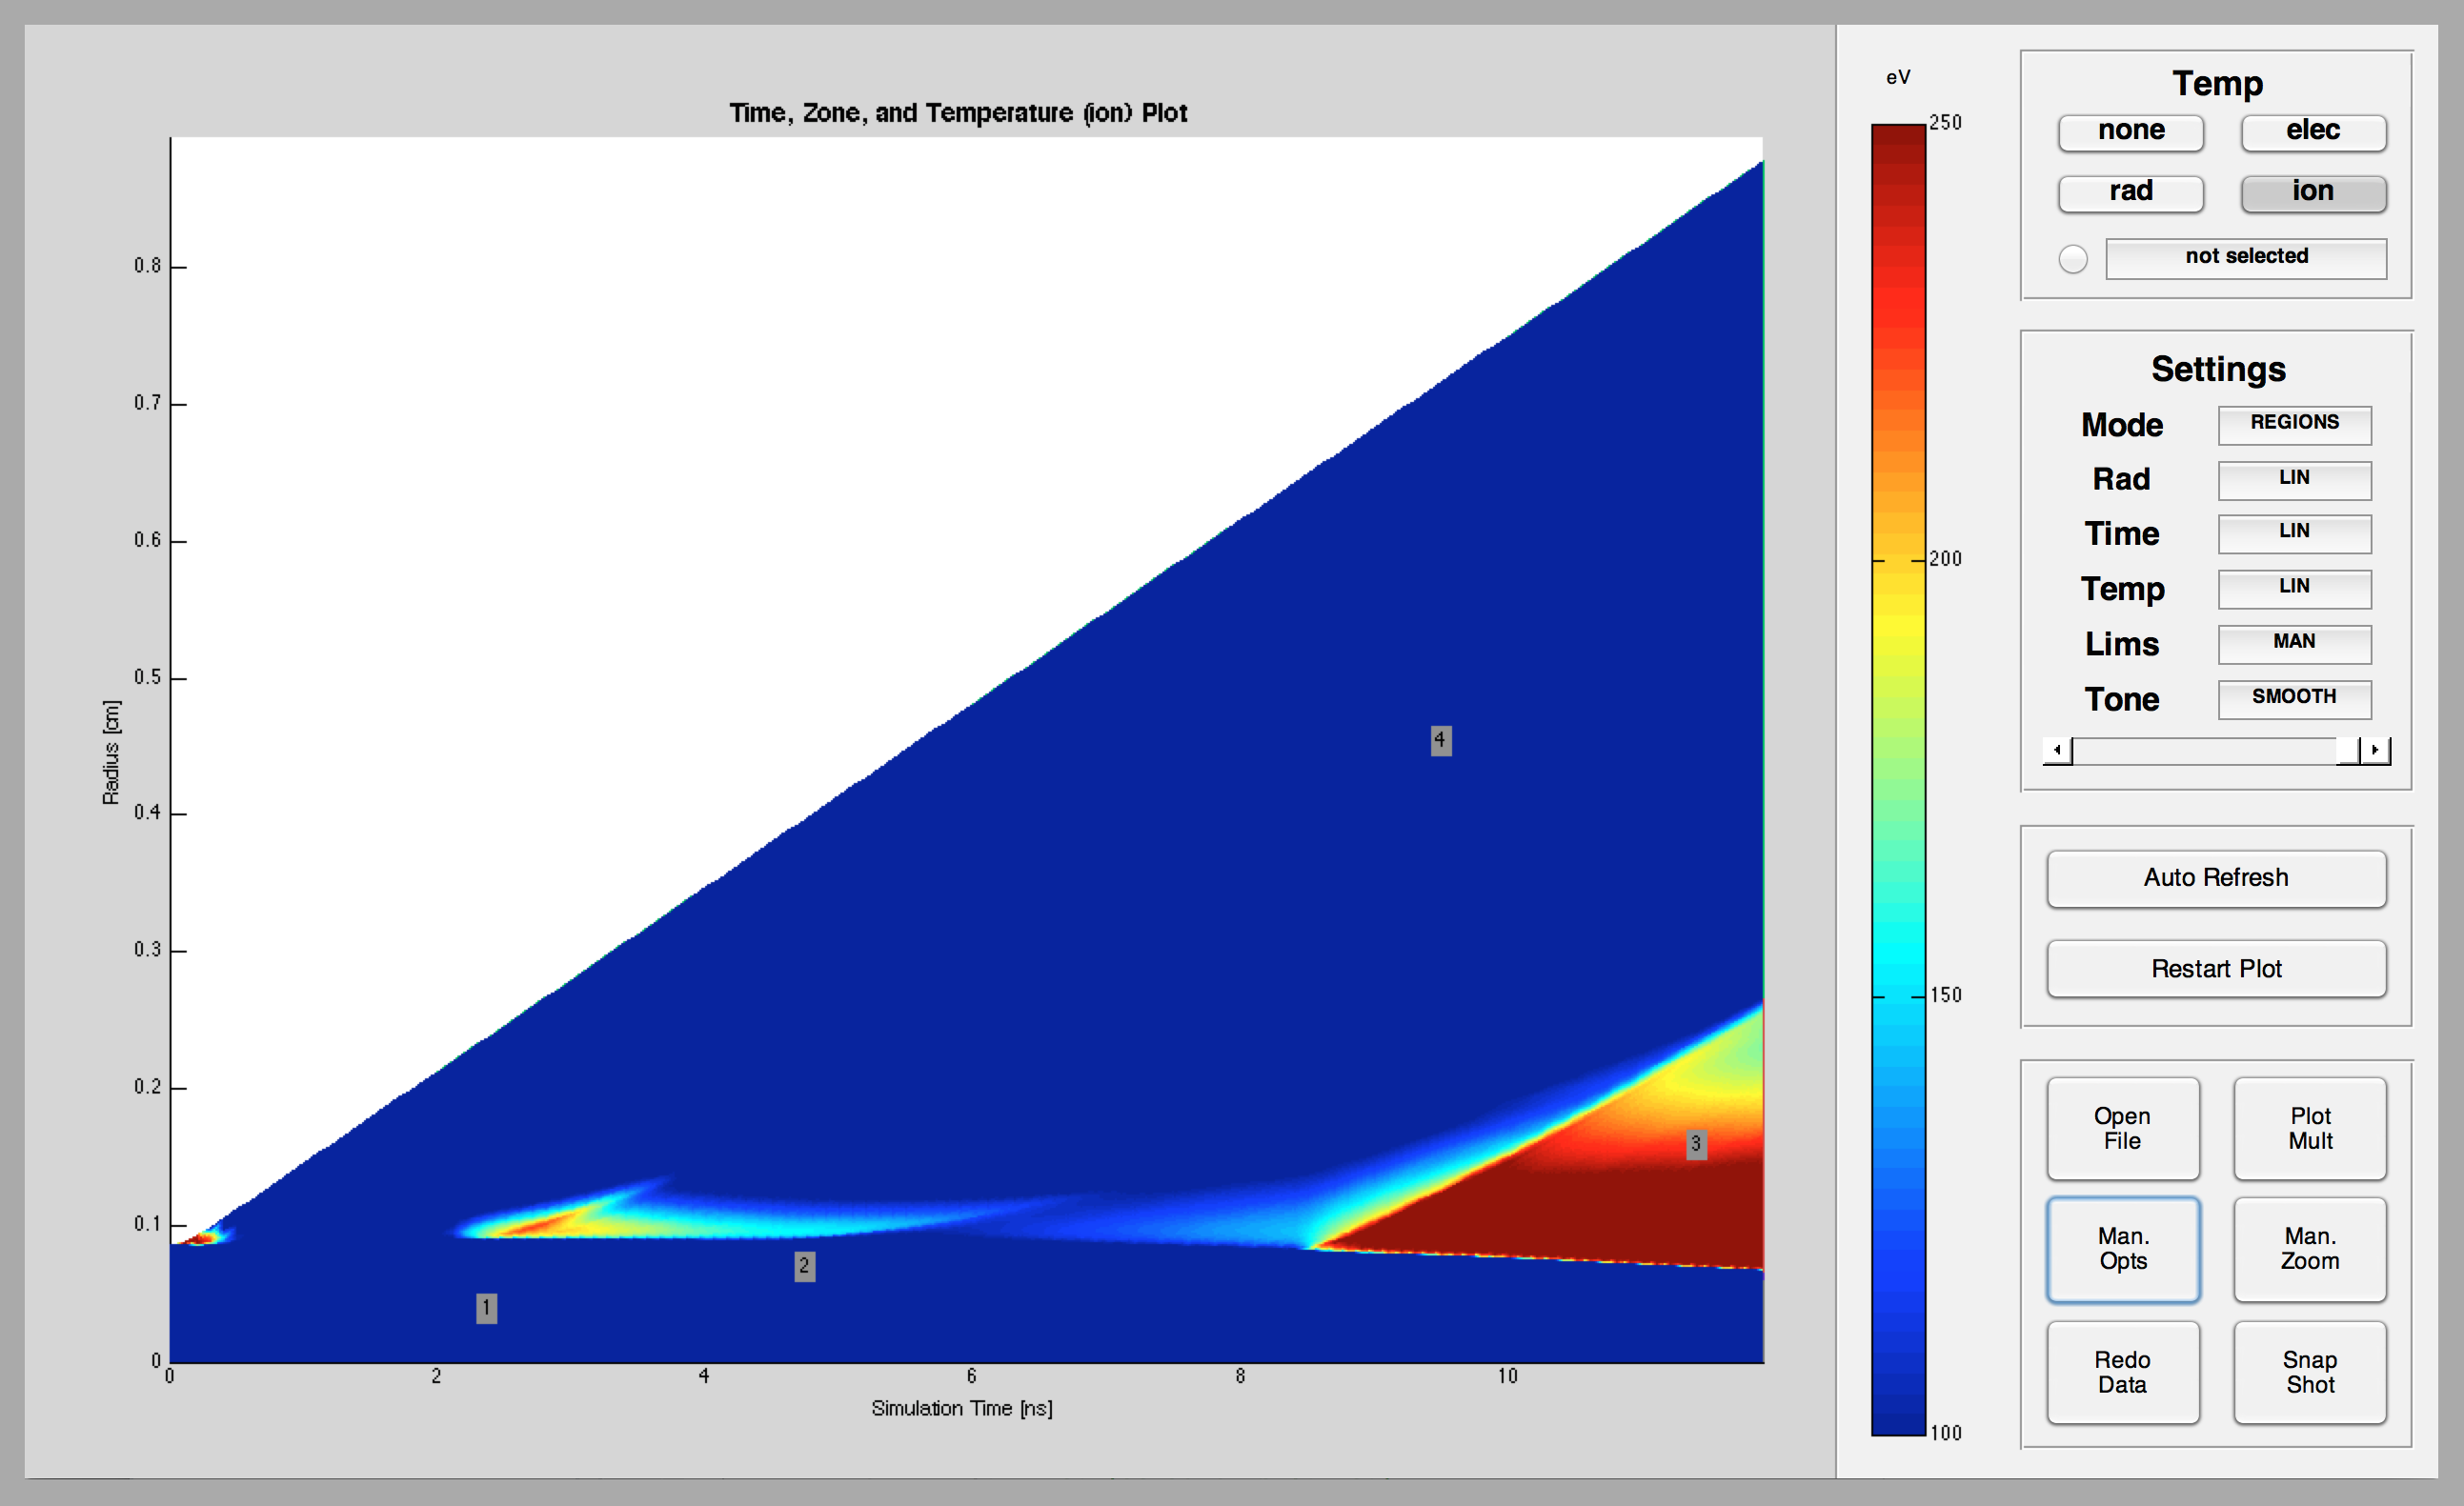
\includegraphics[scale=.23]{graphics/basePlot.png} 
	\caption[The RTT Plotting Function]{ \\ The RTT Plotting Function \\ \captiontitlefinal{\textmd{has an intricate graphical user interface that is designed to give researchers a great degree of freedom when exploring data.  The sidebar shown on the right has four sections of buttons.  The first two sections are involved in changing the plot on the left, while the bottom two deal with special utilities. } } }
	\label{fig:basePlot}
\end{SCfigure}

\subsection{A.0 \ \ Temperature Selection }

The topmost section of buttons on the GUI is involved in changing the overlaying temperature plot.  This connotation of overlaying refers to how temperature variables in Lagrangian codes have values at every spatial position and every temporal position.  

For Bucky, the three temperatures that are most relevant are: the electron temperature, the ion temperature, and the radiation temperature.  However, this notion of temperature was later redefined by extending it to include all variables that have a value for every zone and time.  This can be done by pressing the button labeled 'not selected'.

\subsection{A.1 \ \ Temperature Tone }

The bottommost button in the 'Settings' section is the Tone button.  It changes how the Temperature overlay plot is colored.  The default setting of 'Tone' is 'Smooth'.  Smooth performs an averaging scheme to its discrete data to make it look continuous.  This can prove to be dangerous in some situations because the averaging may be ill-justified.  In those situations - most commonly with logarithmic scales - it is useful to switch the 'Tone' to 'Flat'.  This mode involves no data manipulation.  

\subsection{A.2 \ \ Plot Mode }

The Plot Modes button is the first button in the 'Settings' section.  It refers to how the base Radius Vs. Time plot is done, see Fig.\,\ref{fig:comparison}.  When Mode = 'Regions', the different layers of material are colored as blocks and labeled with numbers.  When Mode = 'Lines', each Lagrangian cell boundary is plotted with region labels attached.

\begin{figure}[h!]%
\centering
\subfloat{
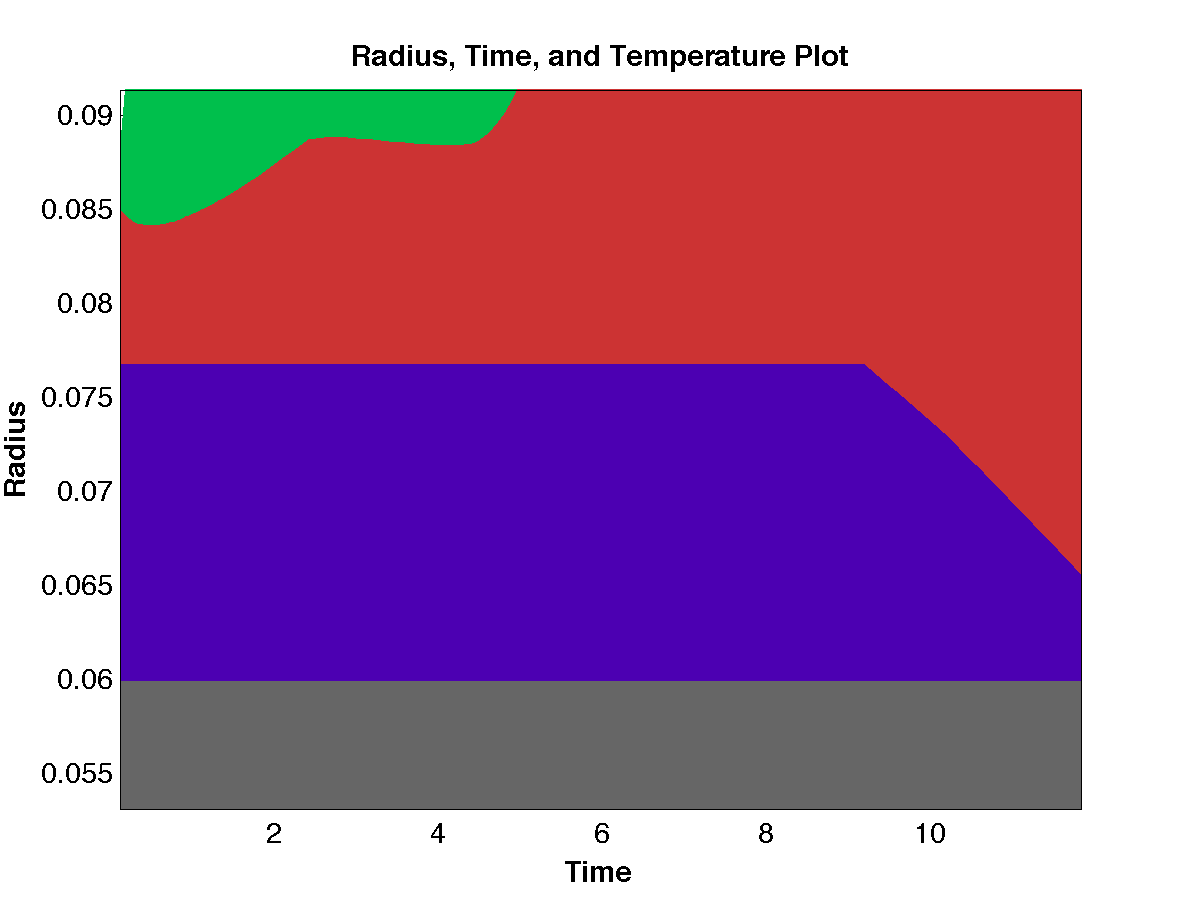
\includegraphics[width=2.5in]{graphics/regions.png} 
}\qquad %
\subfloat{
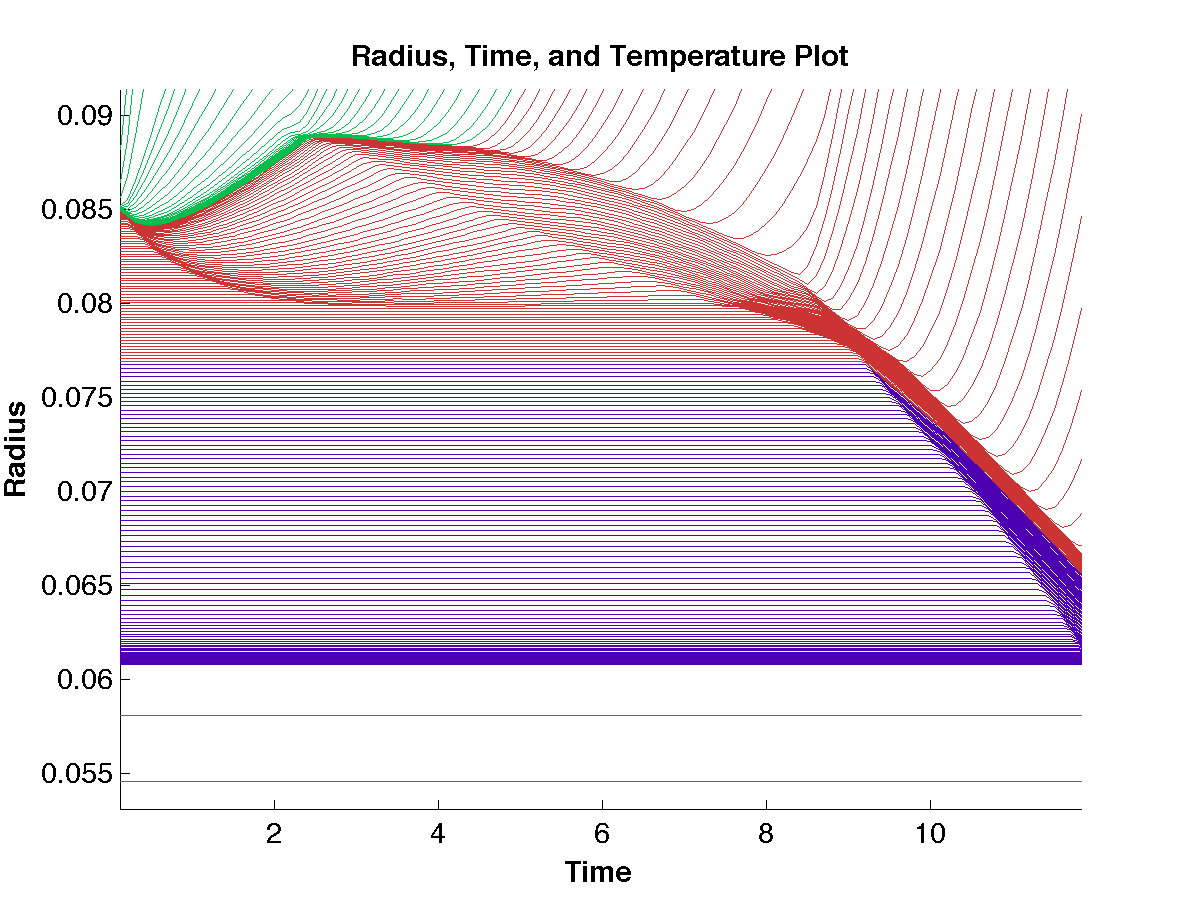
\includegraphics[width=2.5in]{graphics/lines.png} 
}
\caption[Regions Mode vs. Lines Mode]{Comparison of the Regions and Lines Plotting Modes.}
\label{fig:comparison}
\end{figure}

\subsection{A.3 \ \ Dual-Function Slider }

The Slider on the bottom of the 'Settings' section is related to the plot mode button.  When the Mode = 'Regions', the slider changes the transparency of the temperature overlay plot, where the \textit{rightmost} value is equivalent to if the base Radius Vs. Time Plot is completely hidden and the \textit{leftmost} value is equivalent to if 'none' is selected in the 'Temp.' section. When the Mode = 'Lines', the slider changes the number of zone boundary lines that get shown.

\subsection{A.4 \ \ Scales }

The RTT function has three buttons in the 'Settings' section that change the scaling of the problem.  Initially, all three scales - radius, time, and temperature - are set to linear.  They can each be changed to logarithmic and back by clicking their respective buttons.

\subsection{A.5 \ \ Manual Limits }

In addition to changing the scaling of the problem, another common plotting problem is imposing certain limits (i.e. maxima and minima).  This can be done for the radius, the time, and the temperature; however, the temperature is handled differently.  

\begin{wrapfigure}{r}{0.38\textwidth} %[][h!]	
	\vspace{-24pt}
	\centering
	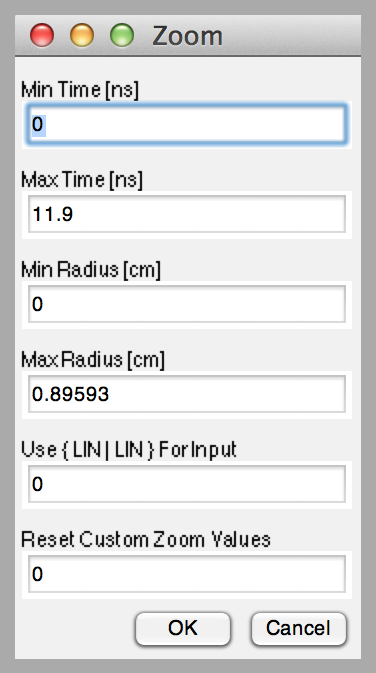
\includegraphics[scale=.83]{graphics/manZoom.png} 
	\vspace{-4pt}
	\caption[Manual Zoom Input Box]{ \small{The Zoom Input Box }\\ \captiontitlefinal{\small{\textmd{gives users a way to zoom to specific areas of the plot. Changing "Lin|Lin" forces these values to be linear, while changing "Reset 'Custom Zoom Values" resets them. } }} }
	\label{fig:manZoom}
\end{wrapfigure}

The Temperature limits involves two buttons that are combined for the other variables.  The first button is \mbox{'Man. Opts'}, which changes the maximum and minimum temperature, while the second button is 'Lims' in the 'Settings' section.  Initially, the 'Lims' button is set to 'Auto', but can be changed to 'Manual'.  The 'Manual' setting changes the temperature limits from the automatically chosen ones to the values inputted in \mbox{'Man. Opts'}.  By default, these limits are 0.1 eV and 200 eV.

For Radius and Time, the manual limits are controlled with the 'Man. Zoom' button.  The term manual refers to how it differs from the automatic zoom that is imposed on the plot at the beginning of the program.  Manual zooming is, thus, changing the minimum and maximum values for the radius and for the time.  With the input box, this can be done in both the current scale and the Linear-Linear scale.  Additionally, the input box allows a way to restart the extrema to their initial values, which are in turn set by the current file's data, see Fig.\,\ref{fig:manZoom}.

\subsection{A.6 \ \ Loading and Reloading Data }

Several buttons in the bottom two sections provide loading and reloading functionality.  'Open File' opens a prompt for users to select a new file to load.  This function is called at the beginning of the RTT function, either implicitly if a data file exists in the local directory, or explicitly with a prompt if no data file is found.  

The 'Redo Data' and the 'Auto Refresh' buttons offer two ways to reload data.  The 'Redo Data' button reopens the current data file.  This is useful for when a run is restarted.  The 'Auto Refresh' reopens the current data file 'n' times at regular intervals of 'm' seconds.  This is useful for when the RTT plot is being used while a Bucky simulation is simultaneously running.  The values of 'n' and 'm' are set inside 'Man. Opts' with default values of 10 seconds and 500 times, respectively.

The 'Restart Plot' button is used to return every selection in the top three sections to their original values. It is located inside the same section as  'Auto Refresh' because it is the only button able to turn off the 'Auto Refresh' effect -- besides by pressing of the \mbox{'Auto Refresh'} button again.  


\subsection{A.7 \ \ Saving the Current Plot to a File }

The 'Snap Shot' button allows researchers to save the current plot to an image.  This is commonly needed for published documents and presentation slides.  This routine has a user select a file name, a destination, and an image type and then saves the plot there.  This function most notably increases the font sizes and removes the background color. 


\subsection{A.8 \ \ Plotting Multiple Files }

The 'Plot Mult' button allows users to open a whole directory of data files and displays their contents inside a scrollable window, see Fig.\,\ref{fig:plotMult}.  The plots produced by this will all share the options set by the user in the top two button sections of the main plot.  

Additionally, when the directory is created by AHAB, every plot's zoom feature is connected together.  This allows users to see the subtle differences in their data (e.g. the arrival time of a specific shock at a certain zone). 

\begin{figure}[h!]	
	\centering
	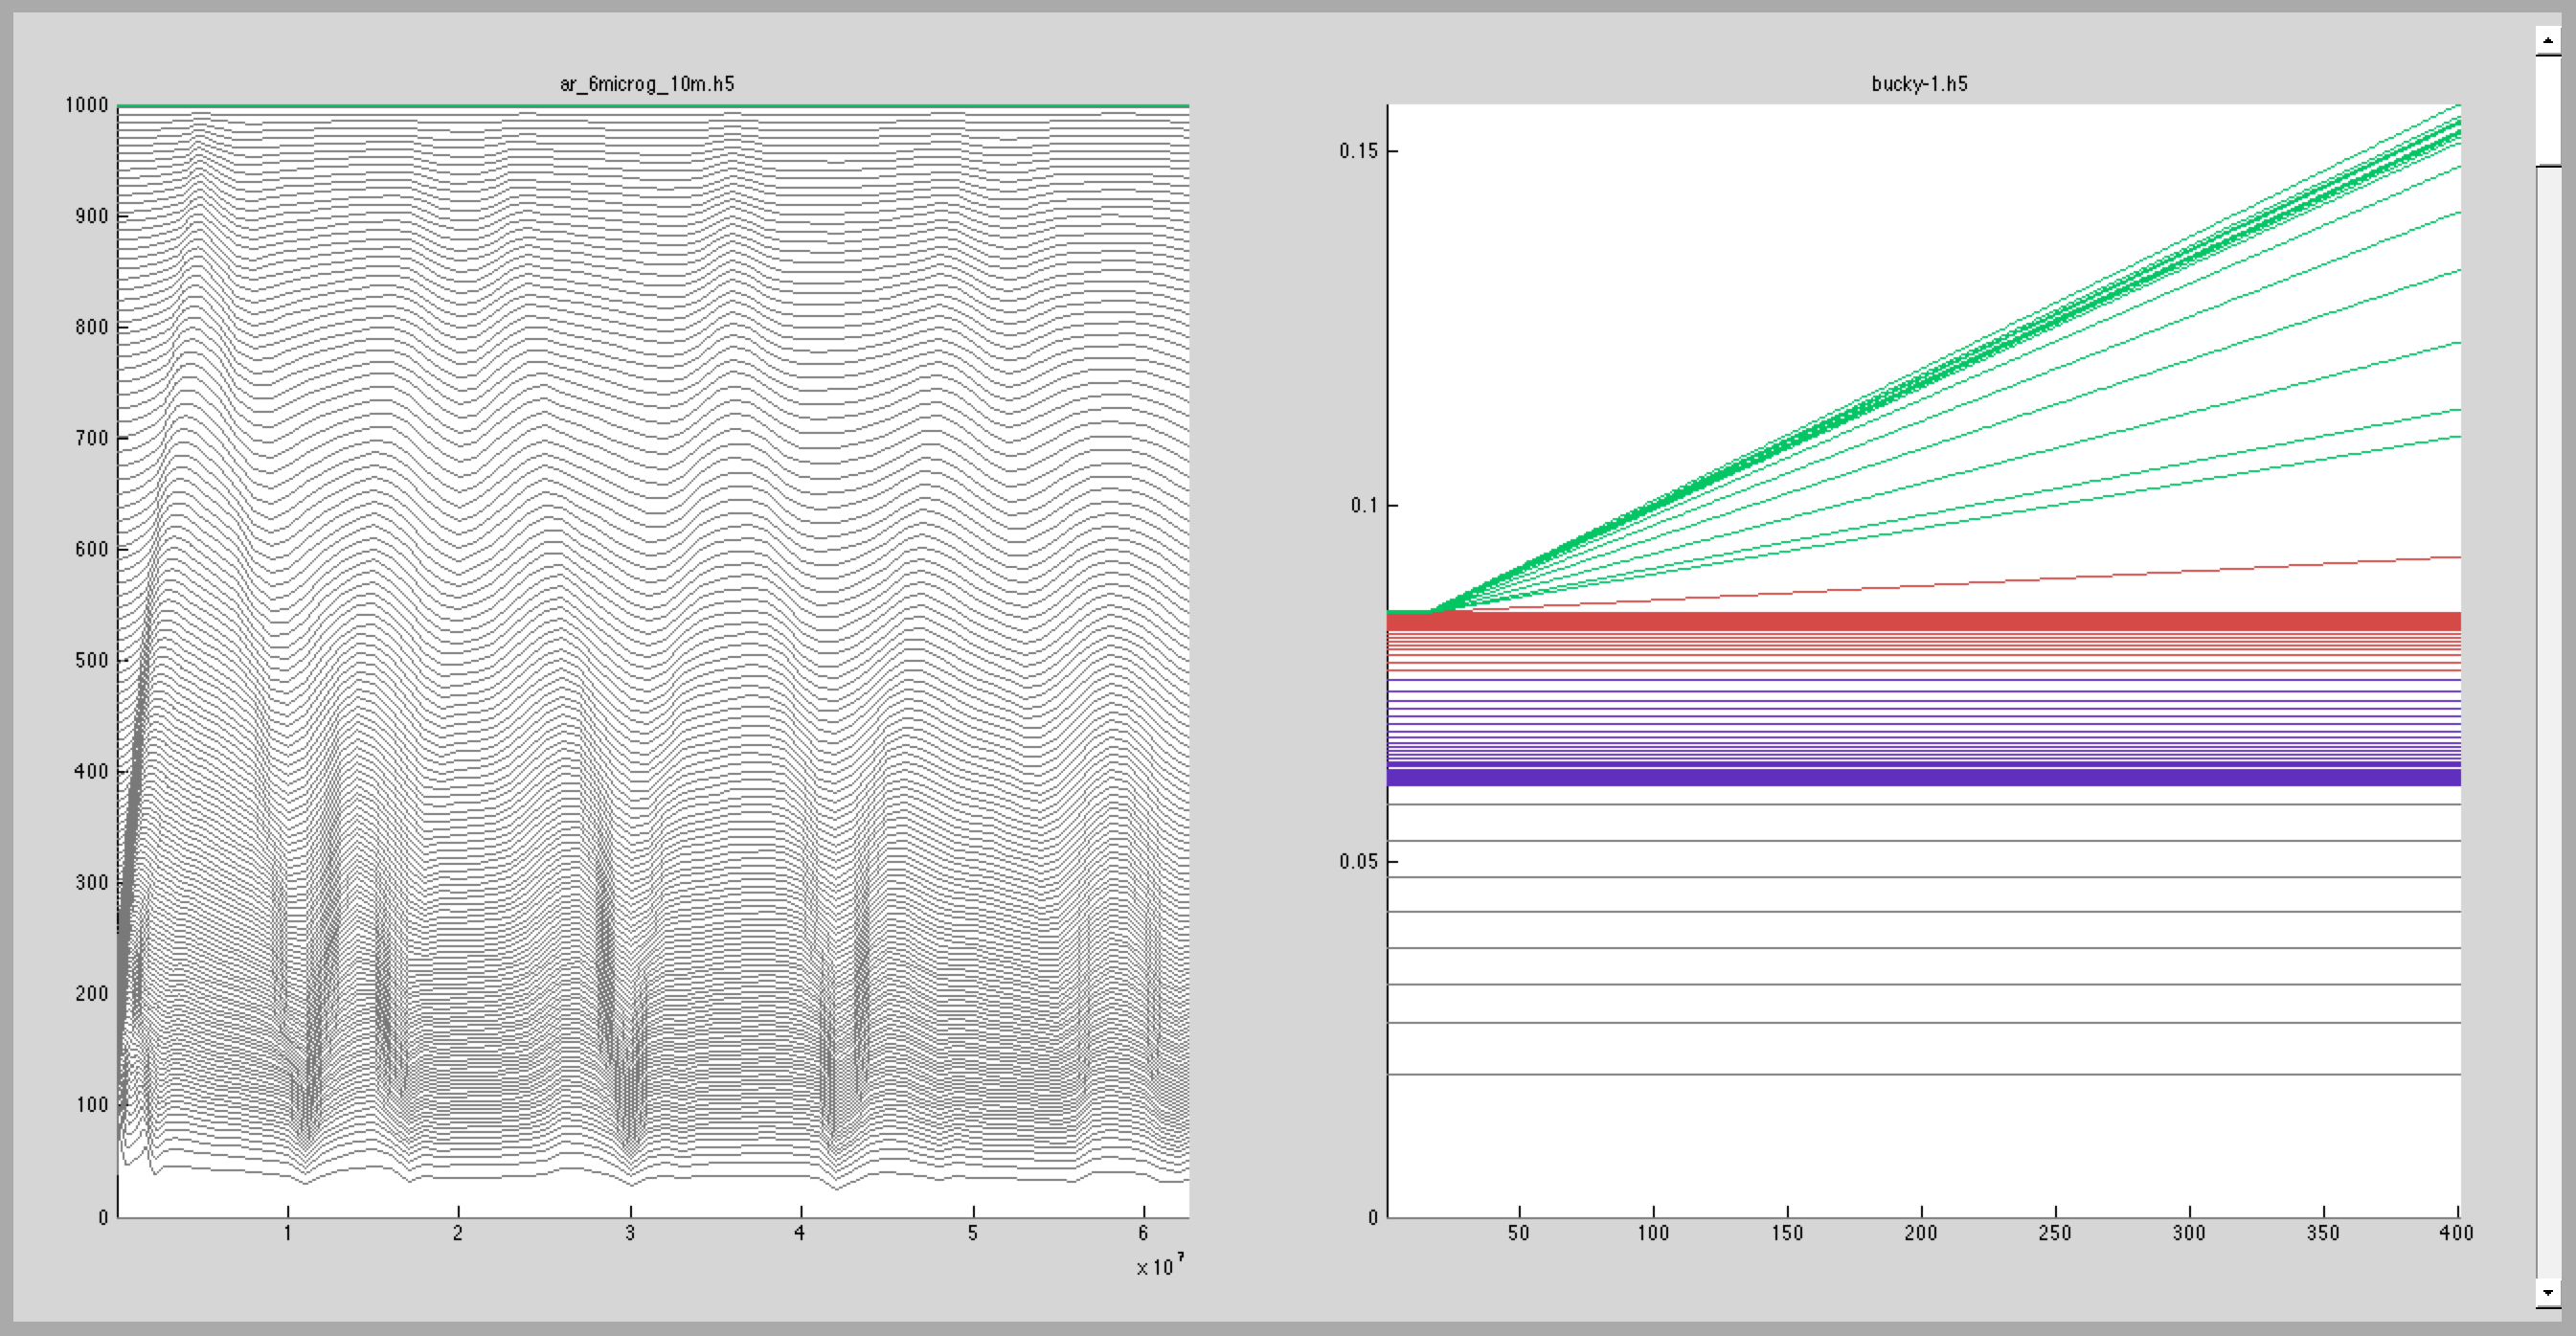
\includegraphics[width=0.68\textwidth]{graphics/plotMult.png} 
	\caption[Plotting Multiple Files]{  The 'Plot Mult' Button \\ \textmd{plots multiple files inside one window. \\ } \tiny{\phantom \\ \phantom} } 
	\label{fig:plotMult}
\end{figure}

\subsection{A.9 \ \ Adding Points to the Plot }

The last feature the RTT plot offers is the "Points Layer."  In the RTT plotting function, each plot is given its own layer (i.e. the Radius Vs. Time Layer, the Temperature Layer, the Text Layer).  The Points Layer is another layer that allows users to add points to the current plot.  These points transform under scale transformations and zooming.  

Additionally, while hovering over the plot in the GUI, a crosshairs is generated; this crosshairs is composed of a vertical line and horizontal line that meet at the cursor and extend to the boundaries of the plot.  When any key besides 'Delete' or 'Escape' is pressed without a modifier (i.e. 'Shift'), a point appears on the plot and has its linear scale coordinates entered on the top left of the screen.  Any number of points can be added to the plot; however, they are all removed when opening a different file. 

\sidecaptionvpos{figure}{b}

\begin{SCfigure}[][h!]	
	\centering
	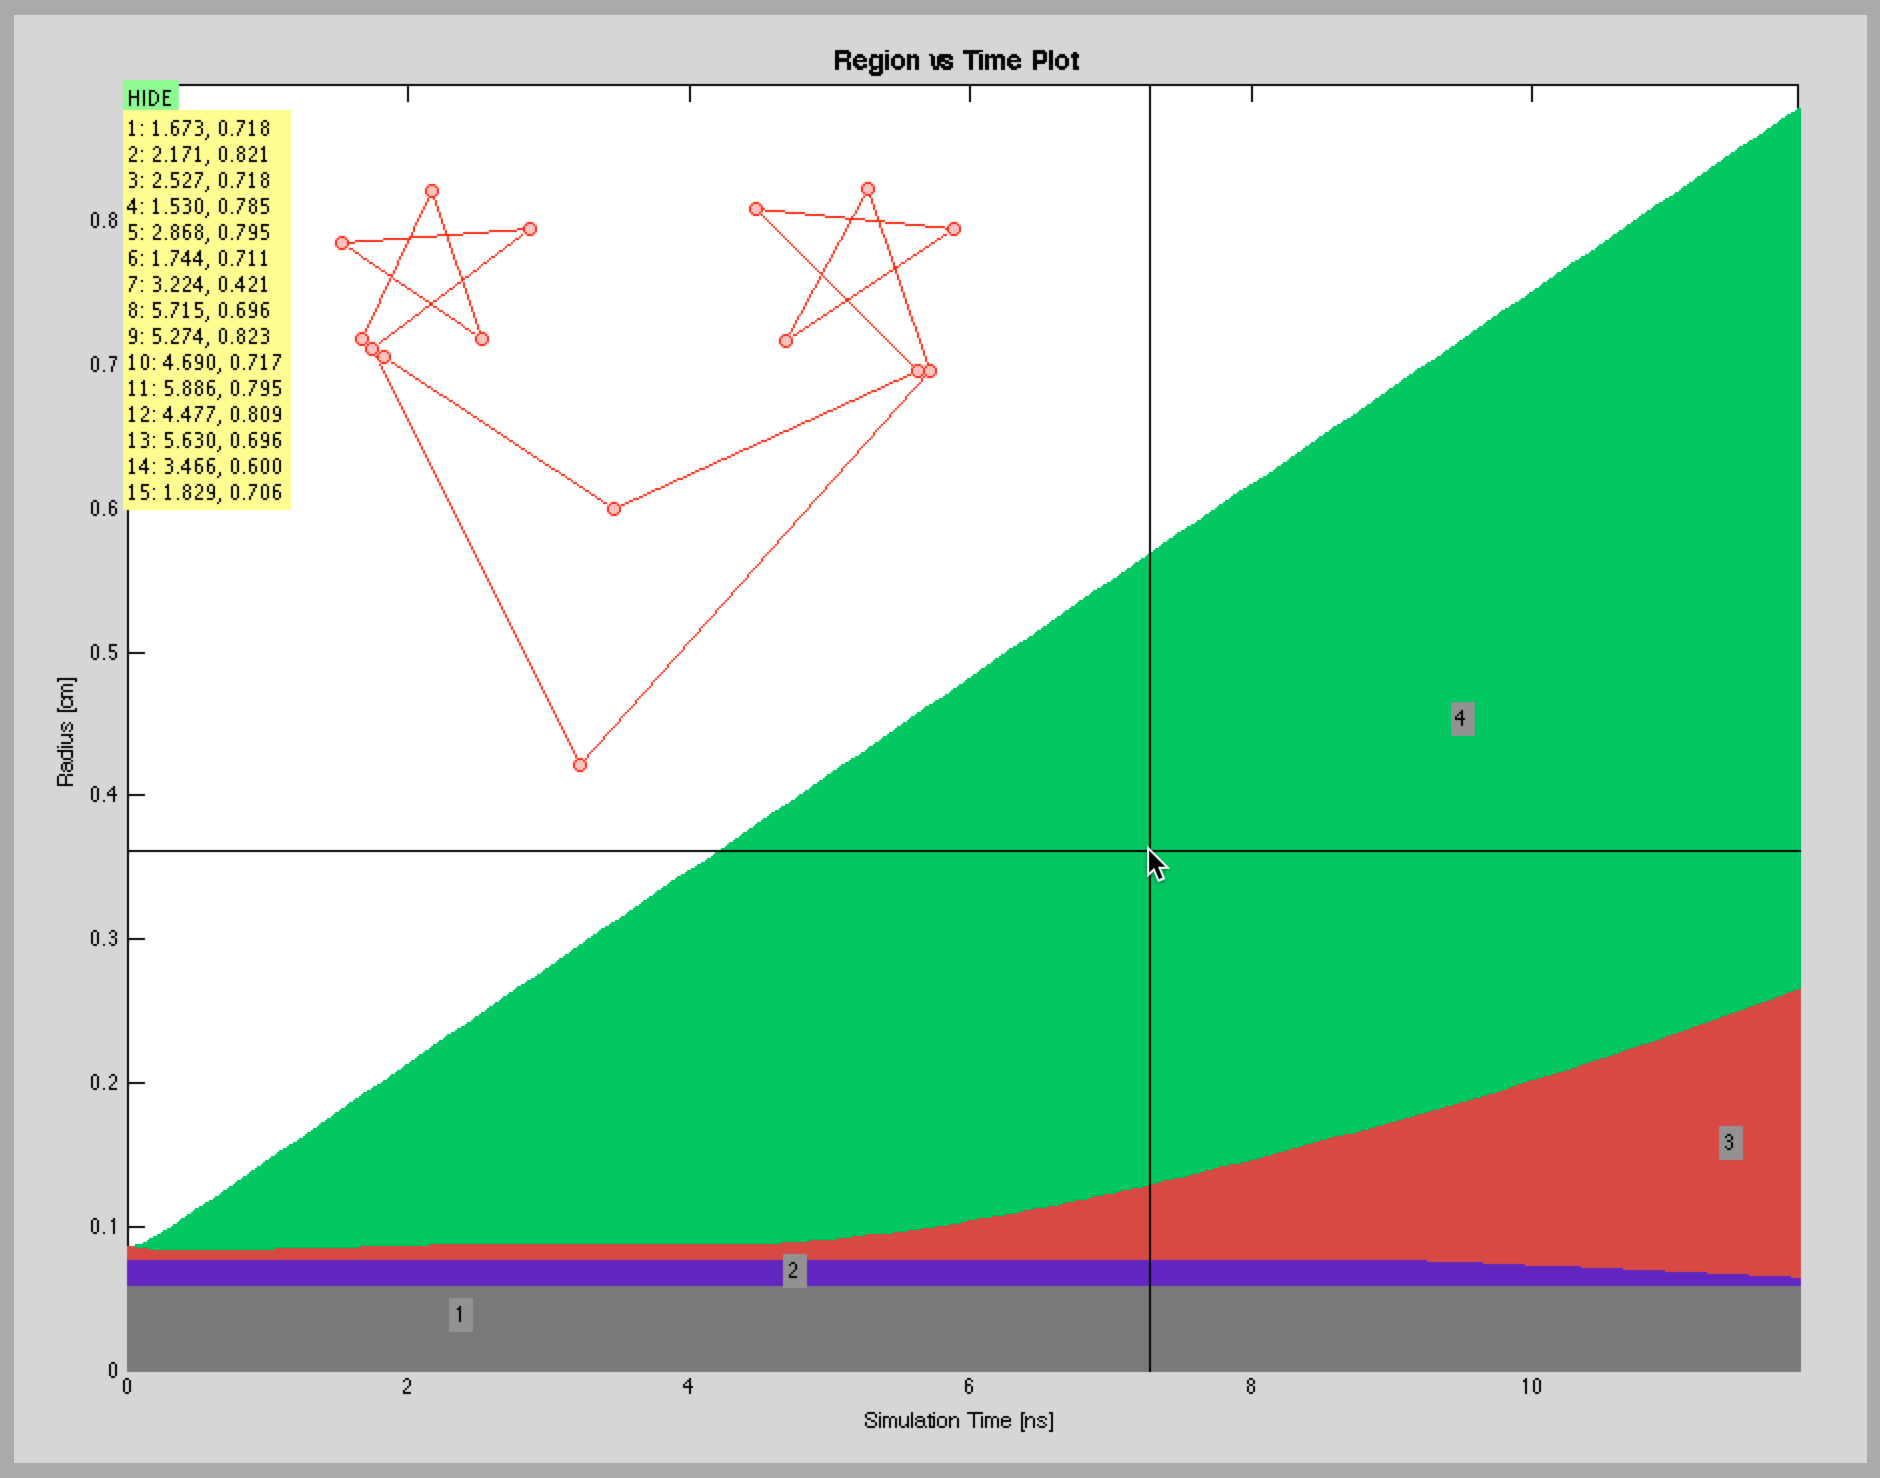
\includegraphics[scale=.24]{graphics/pointsLayer.png} 
	\caption[The Points Layer]{ \\ The Points Layer \\ \captiontitlefinal{\small{\textmd{allows points to be added to the current plot.  This is done by pressing most keyboard keys while hovering over the plot. These points persist through scale changes, but are removed when the file is changed. The coordinates are displayed in the top-left of the plot. } } }}
	\label{fig:pointsLayer}
\end{SCfigure}
